\documentclass[a4paper,12pt,french]{article}
\usepackage[margin=2cm]{geometry}
\usepackage[thinfonts]{uglix2}
\nouveaustyle
\begin{document}
\titre{DM1}{NSI2}{2021}


\begin{center}
\textit{Ceci est une adaptation d'un exercice de deuxième année de BTS SIO.}\\[2em]

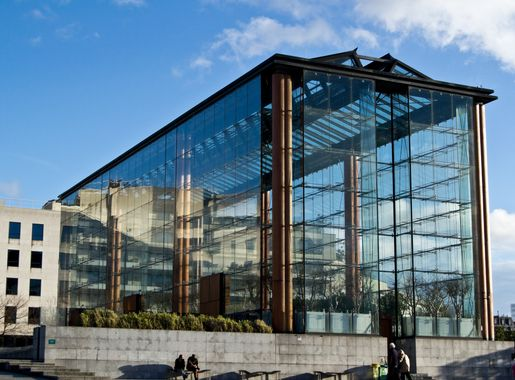
\includegraphics[width=6cm]{img/serres}
\end{center}
Les serres du jardin Citroën (parc situé dans le 15\eme arrondissement de Paris) comprennent des plantes rares sous nos climats.\\
Afin de permettre une bonne croissance de ces plantes, des vaporisateurs d'eau sont installés auprès des plantes : chaque vaporisateur se met en marche automatiquement à une fréquence particulière selon la région d'origine (unique) de la plante.\\
Une plante peut se trouver dans plusieurs serres et une serre peut regrouper des plantes de plusieurs régions.\\
Selon l'emplacement de la serre (en fait, selon son degré d'ensoleillement) et la région d'origine d'une plante, la fréquence de vaporisation va varier.\\
On souhaite réaliser un MCD pour ensuite produire une BDD qui nous permettra de connaître la liste des plantes se trouvant dans une serre, la fréquence de vaporisation pour une serre suivant la région concernée \textit{et c\ae tera}.

Pour nous aider on dispose des informations suivantes (non exhaustives bien entendu).

\begin{center}
\textbf{Liste des plantes de la serre n°1}\\[1em]

\begin{tabular}{|c|c|c|}
\hline\rowcolor{orange@color}
\color{white}\textbf{numéro de plante} & \color{white}\textbf{nom} & \color{white}\textbf{provenance} \\
\hline
1543 & Tabilga & Afrique équatoriale \\
\hline
2541 & Locidus & Austalie \\
\hline
1458 & Bananier & Antilles \\
\hline
1462 & Bananier & Australie \\
\hline
... & ... & ... \\
\hline
\end{tabular}
\end{center}
\begin{center}
\textbf{Liste des plantes de la serre n°2}\\[1em]

\begin{tabular}{|c|c|c|}
\hline\rowcolor{orange@color}
\color{white}\textbf{numéro de plante} & \color{white}\textbf{nom} & \color{white}\textbf{provenance} \\
\hline
1483 & Cacaoyer & Afrique tropicale \\
\hline
3462 & Bananier & Australie \\
\hline
3549 & Coranil & Amazonie \\
\hline
... & ... & ... \\
\hline
\end{tabular}
\end{center}
\newpage
\begin{center}
\textbf{Fréquences de vaporisation}\\[1em]

\begin{tabular}{|c|c|c|}
\hline\rowcolor{orange@color}
\color{white}\textbf{numéro de serre} & \color{white}\textbf{région} & \color{white}\textbf{durée entre deux vaporisations} \\
\hline
1 & Afrique équatoriale & 15 min  \\
\hline
1 & Antilles & 10 min \\
\hline
2 & Afrique équatoriale & 12 min \\
\hline
3 & Amazonie & 7 min \\
\hline
... & ... & ... \\
\hline
\end{tabular}
\end{center}

\textbf{Indications :} On pourra considérer les entités
\begin{itemize}
\item \textbf{Plante}
\item \textbf{Serre}
\item \textbf{Region}
\end{itemize}
et les associations
\begin{itemize}
\item \textbf{Est\_originaire\_de}
\item  \textbf{Est\_situee\_dans}
\item   \textbf{Vaporiser}\textbf{}
\end{itemize}


\end{document}